\chapter{Dominating Set}

Rishnak was pleased to find Ajur and Jura, who were on their way to the water fountain. Rishnak told them that placing a water fountain is an interesting graph-theoretic problem.

Ajur shrugged his shoulders and said, ``How so?''

Rishnak said, ``Let me explain by starting with a new concept.  A \textit{dominating set} of graph~$G=(V,E)$ is a subset of vertices, say~$D$, such that every vertex in~$V-D$---this means a vertex~$x\in V$ and~$x\notin D$---is adjacent to some vertex in~$D$.'' \index{dominating set}

Ajur frowned, not yet understanding.

Realizing his definition was a bit dense, Rishnak waved his hands and a graph appeared [Figure~\ref{18g1}]. He said, ``The vertices in dominating set~$D$ are shown in orange.''

\begin{figure}
\begin{center}
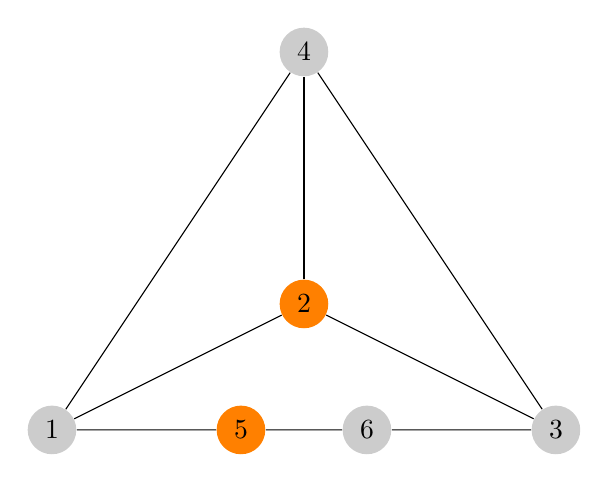
\begin{tikzpicture}
  [scale=.8,auto=left,every node/.style={circle,fill=black!20}]
  \node (n1) at (-1,7) {1};
  \node (n2)[fill=orange] at (3,9)  {2};
  \node (n3) at (7,7)  {3};
  \node (n4) at (3,13)  {4};
  \node (n5)[fill=orange] at (2,7) {5};
  \node (n6) at (4,7) {6};
 \foreach \from/\to in {n1/n2,n2/n3,n2/n4,n1/n4,n3/n4,n1/n5,n5/n6,n6/n3}
    \draw (\from) -- (\to);
\end{tikzpicture}
\caption{A graph in which vertices in dominating set~$D$ are shown in orange; each vertex that is not orange is adjacent to one of the orange vertices}\label{18g1}
\end{center}
\end{figure}

Ajur studied the graph.

Rishnak continued, ``You might think that the dominating set and vertex cover problems seem similar, but they are not the same. In a vertex cover, every edge is incident on one of the vertices in the vertex cover, but in a dominating set, not every vertex is involved.  So in general, we want to find the minimum dominating set.''

Ajur started to see the connection between placing a water fountain and the dominating set.\footnote{Do you see the connection yet?}

Rishnak flashed his hands an a familiar graph appeared [Figure~\ref{18g2}]. He said, ``Here is a street map of Royt. Where would you place water fountains with the condition that every junction or corner either has to have a water fountain or has to be adjacent to a water fountain?''

Ajur studied the graph. He rolled the problem around in his, saying out loud, ``So we assume people will always walk at most one edge to reach a water fountain.''

At length, Ajur drew the graph in the dirt and marked the vertices with petals from an orange flower [Figure~\ref{18g3}]. He said, ``This is the same as finding the dominating set.''

\begin{figure}
\begin{center}

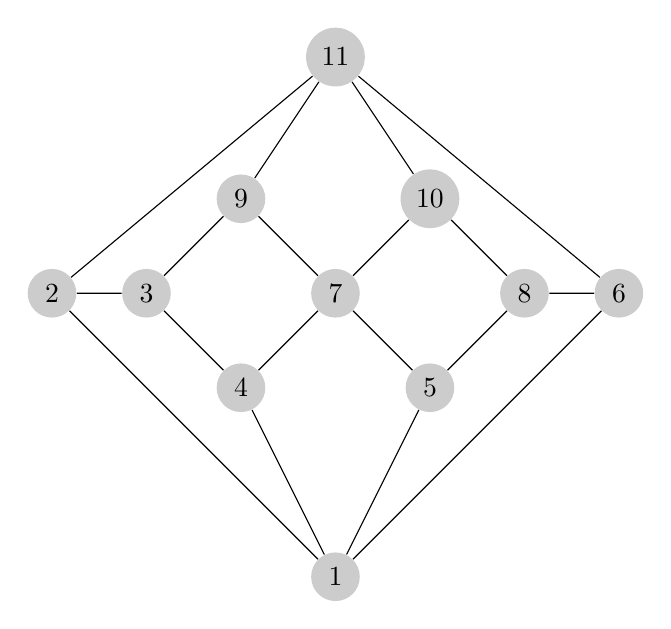
\begin{tikzpicture}
  [scale=.6,auto=left,every node/.style={circle,fill=black!20}]
  \node (n1) at (6,-3) {1};
  \node (n2) at (0,3)  {2};
  \node (n3) at (2,3)  {3};
  \node (n4) at (4,1) {4};
  \node (n5) at (8,1)  {5};
  \node (n6) at (12,3)  {6};
  \node (n7) at (6,3)  {7};
 \node (n8) at (10,3) {8};
  \node (n9) at (4,5)  {9};
  \node (n10) at (8,5)  {10};
  \node (n11) at (6,8)  {11}; 

  \foreach \from/\to in {n1/n2,n1/n4,n1/n5,n1/n6,n2/n3,n2/n11,n3/n4,n3/n9,n4/n7,n5/n7,n5/n8,n6/n8,n6/n11,n7/n9,n7/n10,n8/n10,n9/n11,n10/n11}
    \draw (\from) -- (\to);

\end{tikzpicture}
\caption{A graph representing the streets of Royt for which we wish to place a minimal number of water fountains such that every junction (vertex) either has a water fountain or is adjacent to a water fountain}\label{18g2}
\end{center}
\end{figure}

\begin{figure}
\begin{center}

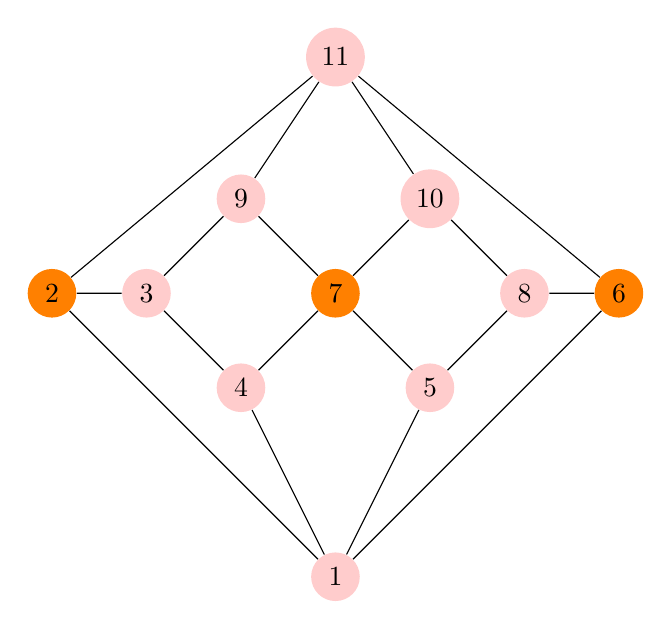
\begin{tikzpicture}
  [scale=.6,auto=left,every node/.style={circle,fill=red!20}]
  \node (n1) at (6,-3) {1};
  \node (n2)[fill=orange] at (0,3)  {2};
  \node (n3) at (2,3)  {3};
  \node (n4) at (4,1) {4};
  \node (n5) at (8,1)  {5};
  \node (n6)[fill=orange] at (12,3)  {6};
  \node (n7)[fill=orange] at (6,3)  {7};
 \node (n8) at (10,3) {8};
  \node (n9) at (4,5)  {9};
  \node (n10) at (8,5)  {10};
  \node (n11) at (6,8)  {11}; 

  \foreach \from/\to in {n1/n2,n1/n4,n1/n5,n1/n6,n2/n3,n2/n11,n3/n4,n3/n9,n4/n7,n5/n7,n5/n8,n6/n8,n6/n11,n7/n9,n7/n10,n8/n10,n9/n11,n10/n11}
    \draw (\from) -- (\to);

\end{tikzpicture}
\caption{The graph from Figure~\ref{18g2} with water fountains placed at vertices~2, 6, and~7, which form a dominating set}\label{18g3}
\end{center}
\end{figure}

\begin{figure}
\begin{center}

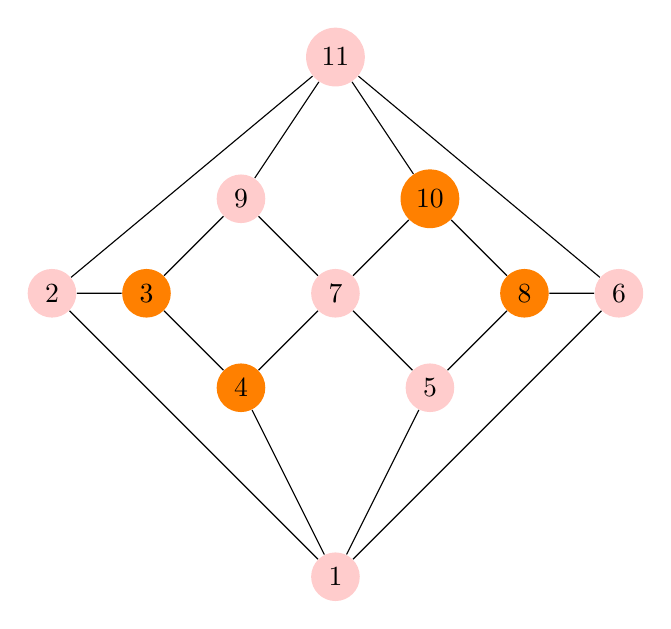
\begin{tikzpicture}
  [scale=.6,auto=left,every node/.style={circle,fill=red!20}]
  \node (n1) at (6,-3) {1};
  \node (n2) at (0,3)  {2};
  \node (n3)[fill=orange] at (2,3)  {3};
  \node (n4)[fill=orange] at (4,1) {4};
  \node (n5) at (8,1)  {5};
  \node (n6) at (12,3)  {6};
  \node (n7) at (6,3)  {7};
 \node (n8) [fill=orange]at (10,3) {8};
  \node (n9) at (4,5)  {9};
  \node (n10)[fill=orange] at (8,5)  {10};
  \node (n11) at (6,8)  {11}; 

  \foreach \from/\to in {n1/n2,n1/n4,n1/n5,n1/n6,n2/n3,n2/n11,n3/n4,n3/n9,n4/n7,n5/n7,n5/n8,n6/n8,n6/n11,n7/n9,n7/n10,n8/n10,n9/n11,n10/n11}
    \draw (\from) -- (\to);

\end{tikzpicture}
\caption{The graph from Figure~\ref{18g2} with total dominating set vertices~3, 4, 8, and~10 shown in orange}\label{18g4}
\end{center}
\end{figure}

\begin{figure}
\begin{center}
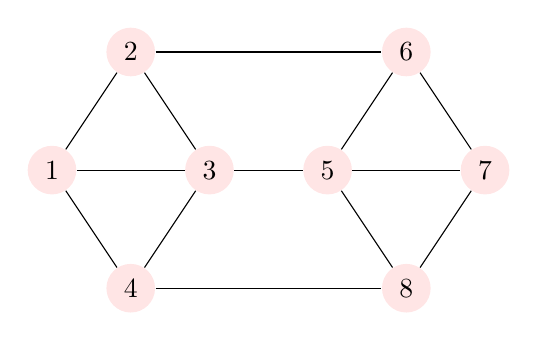
\begin{tikzpicture}
  [scale=.5,auto=left,every node/.style={circle,fill=red!10}]
  \node (n1) at (0,0) {1};
  \node (n2) at (2,3)  {2};
  \node (n3) at (4,0)  {3};
  \node (n4) at (2,-3) {4};
  \node (n5) at (7,0) {5};
  \node (n6) at (9,3)  {6};
  \node (n7) at (11,0)  {7};
  \node (n8) at (9,-3) {8};

  \foreach \from/\to in {n1/n2,n1/n3,n1/n4,n2/n3,n2/n6, n3/n4, n3/n5, n4/n8, n5/n6,n5/n8,n5/n7,n6/n7,n7/n8}
    \draw (\from) -- (\to);

\end{tikzpicture}

\caption{For this graph, where can we place water fountains such that each vertex either has a water fountain or is adjacent to a water fountain?}\label{18q1}
\end{center}
\end{figure}

Rishnak smiled. He said, ``Excellent work. Now let me introduce the concept of a \textit{total dominating set}, which is a variation of the dominating set problem. Total dominating set~$D_T$ of graph~$G=(V,E)$ is a set of vertices for which every vertex~$v\in V$ is adjacent to some vertex in~$D_T$. The dominating set~$\{2,6,7\}$ that you came up with for our map of Royt is not a total dominating set because vertex~2 is not adjacent to any of vertices in~$\{2,6,7\}$.\footnote{A vertex is not considered to be adjacent to itself.} What do you think the total dominating set is for Royt?'' \index{total dominating set}

Ajur had to think hard about this, studying the graph in front of him. Finally, he said, ``I think vertices~3, 4, 7, 8, and~10 form a total dominating set.''

Rishnak said, ``Not bad, Ajur. We can remove vertex~7 from your answer and we have a minimum total dominating set.'' He flashed his hands and some of the vertices of the graph of Royt changed colors [Figure~\ref{18g4}].

Ajur nodded and said, ``I see.''

\newpage
\subsection*{Question for the sixteenth day}
Rishnak said, ``And with that, let us move on to the question for the sixteenth day. For this new graph''---Rishnak flashed his hands and a new graph materialized in the air [Figure~\ref{18q1}]---``can you identify the vertices at which we can place water fountains such that every vertex either has a water fountain or has one adjacent to it?''

\textit{Before you turn the page, try to come up with an answer of your own!}

\newpage
\subsection*{Answer for the sixteenth day}
Ajur copied the graph in the dirt. Within seconds, he had no trouble in placing water fountains at vertices~1 and~7 [Figure~\ref{18qa1}].

\begin{figure}
\begin{center}
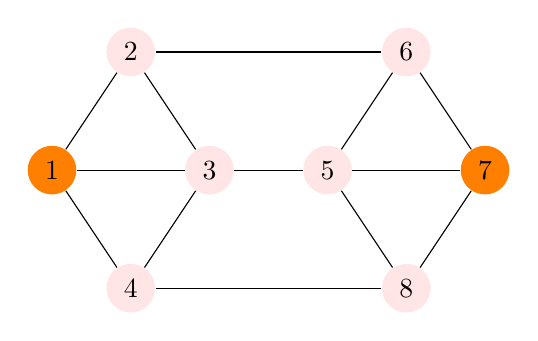
\begin{tikzpicture}
  [scale=.5,auto=left,every node/.style={circle,fill=red!10}]
  \node (n1)[fill=orange] at (0,0) {1};
  \node (n2) at (2,3)  {2};
  \node (n3) at (4,0)  {3};
  \node (n4) at (2,-3) {4};
  \node (n5) at (7,0) {5};
  \node (n6) at (9,3)  {6};
  \node (n7)[fill=orange] at (11,0)  {7};
  \node (n8) at (9,-3) {8};

  \foreach \from/\to in {n1/n2,n1/n3,n1/n4,n2/n3,n2/n6, n3/n4, n3/n5, n4/n8, n5/n6,n5/n8,n5/n7,n6/n7,n7/n8}
    \draw (\from) -- (\to);

\end{tikzpicture}

\caption{The graph from Figure~\ref{18q1} with water fountains, placed at vertices~1 and~7, shown in orange}\label{18qa1}
\end{center}
\end{figure}

By this time, they had walked all the way to the water fountain. Ajur and Jura went to drink from the water fountain, then headed home.
